\chapter{Results}
\label{chap:5}
%
% TODO


We plot the mean and the standard deviation for all kernel runs. One run consists of 10 or 32 trials depending on the experiment. 32 trials are used on cluster runs, because we can use 32 cores to parallelize the run. Due to high variations between iteration steps, all plots are smoothed by a moving mean of five. Also, the standard deviation values are divided by five to maintain readability when three or four different kernel graphs are present in one plot.



\begin{figure}
\centering
\begin{minipage}{.6\textwidth}
  \centering
  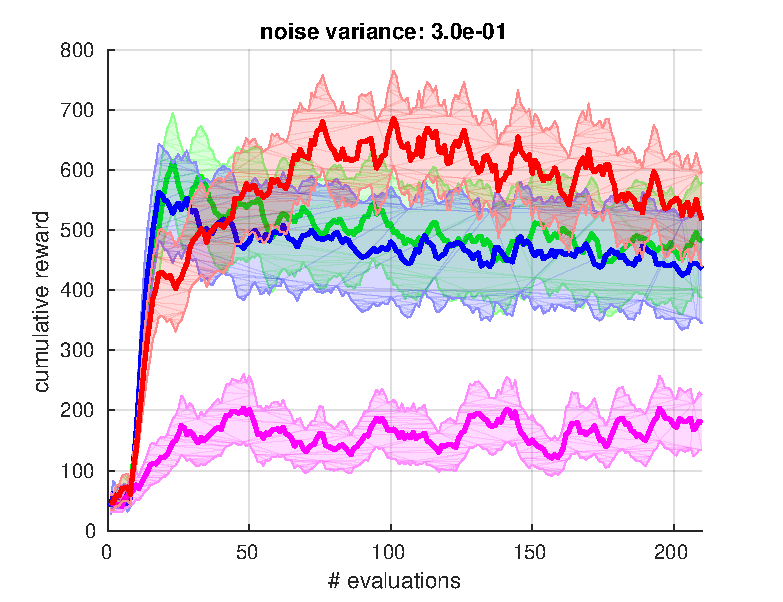
\includegraphics[width=\linewidth]{/home/sebastian/Documents/bscThesis/img/global_cartpole_matlab_32.pdf}
\end{minipage}%
\begin{minipage}{.4\linewidth}
  \centering
  \begin{tabularx}{\linewidth}{|X|l|l|}
      \hline
      kernel & mean(time) & std(time)\\\hline
      trajectory (own work) & 874.0 & 261.0\\\hline
      trajectory (Wilson 2014) & 201.1 & 80.0\\\hline
      matérn 5/2 & 20.7 & 4.8\\\hline
      squared exponential & 19.1 & 4.9\\\hline
  \end{tabularx}
\end{minipage}
\caption{Results of the MATLAB Cart Pole implementation with a continuous action selection policy with the local optimzation. Each kernel graph contains the average over 10 trials.}
\label{fig:cartpolePygym}
\end{figure}

\begin{figure}
\centering
\begin{minipage}{.6\textwidth}
  \centering
  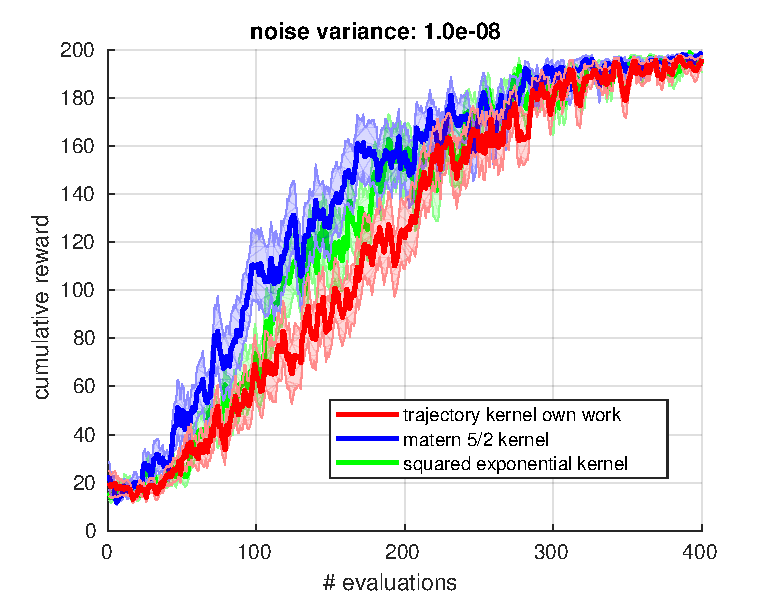
\includegraphics[width=\linewidth]{/home/sebastian/Documents/bscThesis/img/local_cartpole_pygym_10.pdf}
\end{minipage}%
\begin{minipage}{.4\linewidth}
  \centering
  \begin{tabularx}{\linewidth}{|X|l|l|}
      \hline
      kernel & mean(time) & std(time)\\\hline
      trajectory (own work) & 61.6 & 3.5\\\hline
      matérn 5/2 & 8.8 & 1.4\\\hline
      squared exponential & 6.4 & 0.6\\\hline
  \end{tabularx}
\end{minipage}
\caption{Results of the Open AI Cart Pole implementation with a discrete action selection policy with the local optimzation. Each kernel graph contains the average over 10 trials.}
\label{fig:cartpolePygym}
\end{figure}



\begin{figure}[h]
\centering
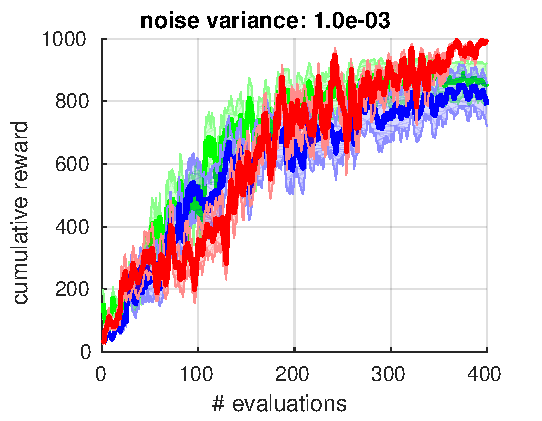
\includegraphics[width=0.4\textwidth]{/home/sebastian/Documents/bscThesis/img/noisecompare/1.pdf}
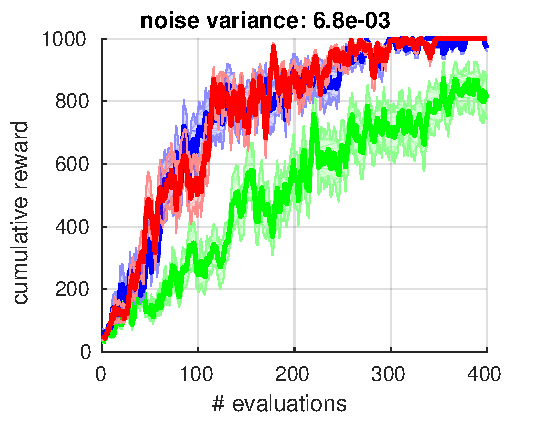
\includegraphics[width=0.4\textwidth]{/home/sebastian/Documents/bscThesis/img/noisecompare/2.pdf}
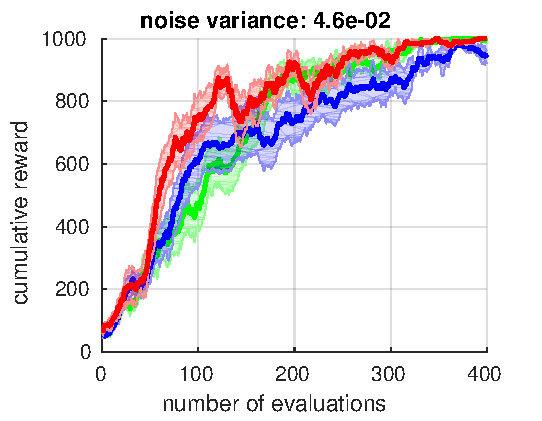
\includegraphics[width=0.4\textwidth]{/home/sebastian/Documents/bscThesis/img/noisecompare/3.pdf}
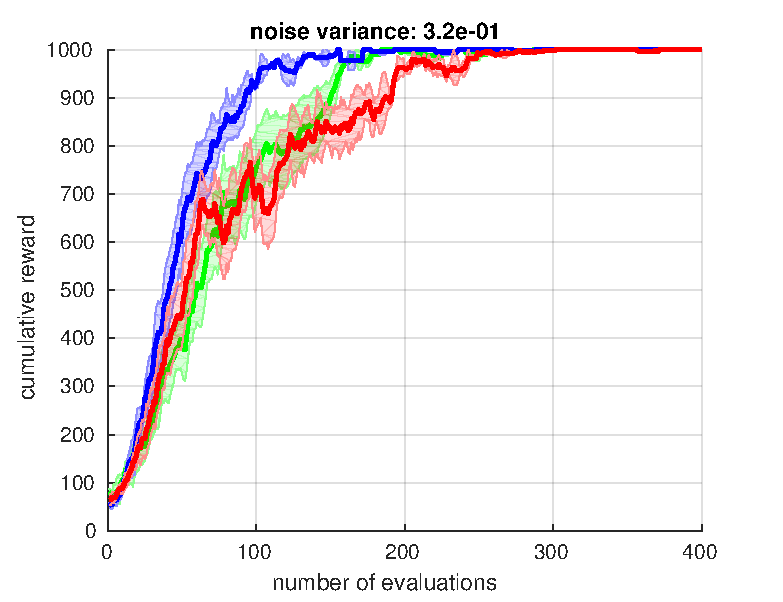
\includegraphics[width=0.4\textwidth]{/home/sebastian/Documents/bscThesis/img/noisecompare/4.pdf}
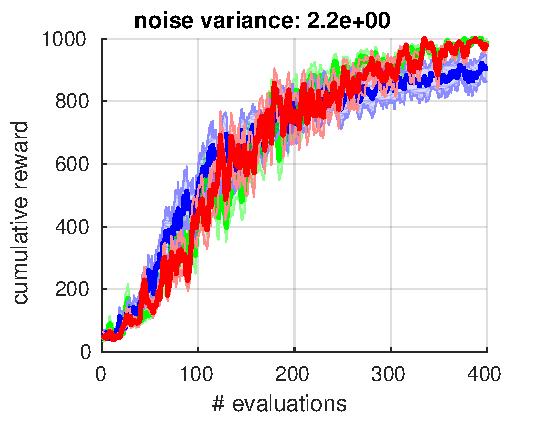
\includegraphics[width=0.4\textwidth]{/home/sebastian/Documents/bscThesis/img/noisecompare/5.pdf}
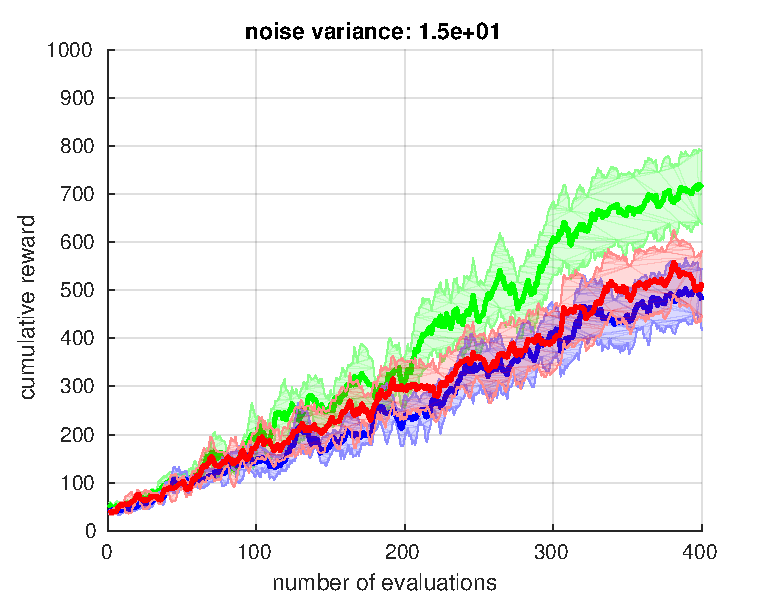
\includegraphics[width=0.4\textwidth]{/home/sebastian/Documents/bscThesis/img/noisecompare/6.pdf}
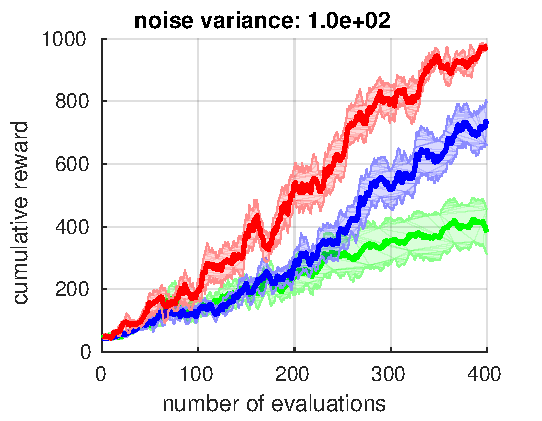
\includegraphics[width=0.4\textwidth]{/home/sebastian/Documents/bscThesis/img/noisecompare/7.pdf}
\raisebox{\height}{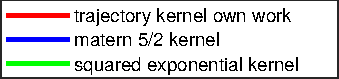
\includegraphics[width=0.4\textwidth]{/home/sebastian/Documents/bscThesis/img/noisecompare/legend.pdf}}

\caption{Noise level comparison on the MATLAB Cart Pole implementation with 1000 time steps on the local Bayesian optimizer. The noise levels are logarithmically spaced and sorted in ascending order from $10^{-3}$ to $10^2$. Each kernel graph contains the average over 5 trials.}
\label{fig:noisecompare}
\end{figure}
